% Options for packages loaded elsewhere
\PassOptionsToPackage{unicode}{hyperref}
\PassOptionsToPackage{hyphens}{url}
\PassOptionsToPackage{dvipsnames,svgnames,x11names}{xcolor}
%
\documentclass[
  letterpaper,
  DIV=11,
  numbers=noendperiod]{scrartcl}

\usepackage{amsmath,amssymb}
\usepackage{iftex}
\ifPDFTeX
  \usepackage[T1]{fontenc}
  \usepackage[utf8]{inputenc}
  \usepackage{textcomp} % provide euro and other symbols
\else % if luatex or xetex
  \usepackage{unicode-math}
  \defaultfontfeatures{Scale=MatchLowercase}
  \defaultfontfeatures[\rmfamily]{Ligatures=TeX,Scale=1}
\fi
\usepackage{lmodern}
\ifPDFTeX\else  
    % xetex/luatex font selection
\fi
% Use upquote if available, for straight quotes in verbatim environments
\IfFileExists{upquote.sty}{\usepackage{upquote}}{}
\IfFileExists{microtype.sty}{% use microtype if available
  \usepackage[]{microtype}
  \UseMicrotypeSet[protrusion]{basicmath} % disable protrusion for tt fonts
}{}
\makeatletter
\@ifundefined{KOMAClassName}{% if non-KOMA class
  \IfFileExists{parskip.sty}{%
    \usepackage{parskip}
  }{% else
    \setlength{\parindent}{0pt}
    \setlength{\parskip}{6pt plus 2pt minus 1pt}}
}{% if KOMA class
  \KOMAoptions{parskip=half}}
\makeatother
\usepackage{xcolor}
\setlength{\emergencystretch}{3em} % prevent overfull lines
\setcounter{secnumdepth}{-\maxdimen} % remove section numbering
% Make \paragraph and \subparagraph free-standing
\makeatletter
\ifx\paragraph\undefined\else
  \let\oldparagraph\paragraph
  \renewcommand{\paragraph}{
    \@ifstar
      \xxxParagraphStar
      \xxxParagraphNoStar
  }
  \newcommand{\xxxParagraphStar}[1]{\oldparagraph*{#1}\mbox{}}
  \newcommand{\xxxParagraphNoStar}[1]{\oldparagraph{#1}\mbox{}}
\fi
\ifx\subparagraph\undefined\else
  \let\oldsubparagraph\subparagraph
  \renewcommand{\subparagraph}{
    \@ifstar
      \xxxSubParagraphStar
      \xxxSubParagraphNoStar
  }
  \newcommand{\xxxSubParagraphStar}[1]{\oldsubparagraph*{#1}\mbox{}}
  \newcommand{\xxxSubParagraphNoStar}[1]{\oldsubparagraph{#1}\mbox{}}
\fi
\makeatother


\providecommand{\tightlist}{%
  \setlength{\itemsep}{0pt}\setlength{\parskip}{0pt}}\usepackage{longtable,booktabs,array}
\usepackage{calc} % for calculating minipage widths
% Correct order of tables after \paragraph or \subparagraph
\usepackage{etoolbox}
\makeatletter
\patchcmd\longtable{\par}{\if@noskipsec\mbox{}\fi\par}{}{}
\makeatother
% Allow footnotes in longtable head/foot
\IfFileExists{footnotehyper.sty}{\usepackage{footnotehyper}}{\usepackage{footnote}}
\makesavenoteenv{longtable}
\usepackage{graphicx}
\makeatletter
\newsavebox\pandoc@box
\newcommand*\pandocbounded[1]{% scales image to fit in text height/width
  \sbox\pandoc@box{#1}%
  \Gscale@div\@tempa{\textheight}{\dimexpr\ht\pandoc@box+\dp\pandoc@box\relax}%
  \Gscale@div\@tempb{\linewidth}{\wd\pandoc@box}%
  \ifdim\@tempb\p@<\@tempa\p@\let\@tempa\@tempb\fi% select the smaller of both
  \ifdim\@tempa\p@<\p@\scalebox{\@tempa}{\usebox\pandoc@box}%
  \else\usebox{\pandoc@box}%
  \fi%
}
% Set default figure placement to htbp
\def\fps@figure{htbp}
\makeatother
% definitions for citeproc citations
\NewDocumentCommand\citeproctext{}{}
\NewDocumentCommand\citeproc{mm}{%
  \begingroup\def\citeproctext{#2}\cite{#1}\endgroup}
\makeatletter
 % allow citations to break across lines
 \let\@cite@ofmt\@firstofone
 % avoid brackets around text for \cite:
 \def\@biblabel#1{}
 \def\@cite#1#2{{#1\if@tempswa , #2\fi}}
\makeatother
\newlength{\cslhangindent}
\setlength{\cslhangindent}{1.5em}
\newlength{\csllabelwidth}
\setlength{\csllabelwidth}{3em}
\newenvironment{CSLReferences}[2] % #1 hanging-indent, #2 entry-spacing
 {\begin{list}{}{%
  \setlength{\itemindent}{0pt}
  \setlength{\leftmargin}{0pt}
  \setlength{\parsep}{0pt}
  % turn on hanging indent if param 1 is 1
  \ifodd #1
   \setlength{\leftmargin}{\cslhangindent}
   \setlength{\itemindent}{-1\cslhangindent}
  \fi
  % set entry spacing
  \setlength{\itemsep}{#2\baselineskip}}}
 {\end{list}}
\usepackage{calc}
\newcommand{\CSLBlock}[1]{\hfill\break\parbox[t]{\linewidth}{\strut\ignorespaces#1\strut}}
\newcommand{\CSLLeftMargin}[1]{\parbox[t]{\csllabelwidth}{\strut#1\strut}}
\newcommand{\CSLRightInline}[1]{\parbox[t]{\linewidth - \csllabelwidth}{\strut#1\strut}}
\newcommand{\CSLIndent}[1]{\hspace{\cslhangindent}#1}

\usepackage{booktabs}
\usepackage{longtable}
\usepackage{array}
\usepackage{multirow}
\usepackage{wrapfig}
\usepackage{float}
\usepackage{colortbl}
\usepackage{pdflscape}
\usepackage{tabu}
\usepackage{threeparttable}
\usepackage{threeparttablex}
\usepackage[normalem]{ulem}
\usepackage{makecell}
\usepackage{xcolor}
\KOMAoption{captions}{tableheading}
\makeatletter
\@ifpackageloaded{caption}{}{\usepackage{caption}}
\AtBeginDocument{%
\ifdefined\contentsname
  \renewcommand*\contentsname{Table of contents}
\else
  \newcommand\contentsname{Table of contents}
\fi
\ifdefined\listfigurename
  \renewcommand*\listfigurename{List of Figures}
\else
  \newcommand\listfigurename{List of Figures}
\fi
\ifdefined\listtablename
  \renewcommand*\listtablename{List of Tables}
\else
  \newcommand\listtablename{List of Tables}
\fi
\ifdefined\figurename
  \renewcommand*\figurename{Figure}
\else
  \newcommand\figurename{Figure}
\fi
\ifdefined\tablename
  \renewcommand*\tablename{Table}
\else
  \newcommand\tablename{Table}
\fi
}
\@ifpackageloaded{float}{}{\usepackage{float}}
\floatstyle{ruled}
\@ifundefined{c@chapter}{\newfloat{codelisting}{h}{lop}}{\newfloat{codelisting}{h}{lop}[chapter]}
\floatname{codelisting}{Listing}
\newcommand*\listoflistings{\listof{codelisting}{List of Listings}}
\makeatother
\makeatletter
\makeatother
\makeatletter
\@ifpackageloaded{caption}{}{\usepackage{caption}}
\@ifpackageloaded{subcaption}{}{\usepackage{subcaption}}
\makeatother

\usepackage{bookmark}

\IfFileExists{xurl.sty}{\usepackage{xurl}}{} % add URL line breaks if available
\urlstyle{same} % disable monospaced font for URLs
\hypersetup{
  pdftitle={ESRM 6990V Class Project},
  pdfauthor={Henrietta Kadi Tettey-Tawiah},
  colorlinks=true,
  linkcolor={blue},
  filecolor={Maroon},
  citecolor={Blue},
  urlcolor={Blue},
  pdfcreator={LaTeX via pandoc}}


\title{ESRM 6990V Class Project}
\author{Henrietta Kadi Tettey-Tawiah}
\date{}

\begin{document}
\maketitle


\section{TIMSS DATA}\label{timss-data}

\subsection{Introduction: Research Scenario and Research
Questions}\label{introduction-research-scenario-and-research-questions}

The researcher would want to investigate the performance of students in
the United States of America (USA) and Canada based on the 2023
\href{https://timss2023.org/data}{TIMSS} (Trends in International
Mathematics and Science Study) dataset. This analysis focuses on math
performance of 4th grade students using their percentage correct on the
TIMSS math achievement test. In this study, student level factors, home
factors as well as teacher-level factors are explored to identify their
respective impacts on an individual student's math test score.
Specifically, this research;

\begin{enumerate}
\def\labelenumi{\arabic{enumi}.}
\tightlist
\item
  Explores how factors such as gender, country, student confidence among
  others affect the performance of a student on the math test.

  \begin{itemize}
  \tightlist
  \item
    Explore if there are any country-level and/or sex differences in
    math percentage scores. (``How does math performance vary across
    countries and sexes?'')
  \item
    Examines how various teacher characteristics influence student's
    score on the math test
  \end{itemize}
\end{enumerate}

\subsection{Data Analysis}\label{data-analysis}

\subsubsection{Student-Level Analysis}\label{student-level-analysis}

The dataset used in this contained a total of 18369 participants after
data cleaning. The dataset had a total of 373 variables but only 13 are
reported below:

\begin{itemize}
\item
  \textbf{Student\_ID:} Student Identifier
\item
  \textbf{Country:} Country of Participation (CAN = 1, USA = 2)
\item
  \textbf{Sex:} Sex/Gender (1 = Girl, 2 = Boy)
\item
  \textbf{Age :} Age of student
\item
  \textbf{Number\_of\_Home\_Study\_Supports:} Derived from subscale
  measuring resources available to the student at home.
\item
  \textbf{Disorderly\_Behavior:} Scale score from the subscale measuring
  disorderly behavior during math lessons.
\item
  \textbf{Instructional\_Clarity:} Scale score from the subscale
  measuring instructional clarity in mathematics lessons.
\item
  \textbf{Digital\_Self\_Efficacy:} Scale score from the subscale
  measuring digital self-efficacy.
\item
  \textbf{Sense\_of\_School\_Belonging:} Scale score from the subscale
  measuring students sense of school belonging.
\item
  \textbf{Student\_Bullying:} Scale score from the subscale measuring
  student bullying.
\item
  \textbf{Like\_Learning\_Math:} Scale score from the subscale measuring
  if students like learning mathematics.
\item
  \textbf{Confident\_in\_Math:} Scale score from the subscale measuring
  students confidence in mathematics.
\item
  \textbf{Math\_Percent\_Correct}: Students' percent correct on the 2023
  TIMSS Math Achievement Test.
\end{itemize}

The scale scores reported were derived following several steps
including; item parameter estimation, item fit evaluation among others
(Yin and Reynolds 2024).

\paragraph{Data Preparation}\label{data-preparation}

The data preparation stage began with renaming the columns in the
\texttt{Home\_Student} dataset with more descriptive names. After this,
the dataset is cleaned by removing any rows containing missing values
resulting in a final dataset with only complete cases as well as
specifying categorical variables and dropping any unused levels.

\paragraph{Descriptive Statistics}\label{descriptive-statistics}

The total sample size of the Canada and U.S.A. 4th grade students was
22806. However, due to non-response, the sample size used for this
analysis was 18369; 9351 girls and 9018 boys. There were more Canadian
4th Grade students compared to the U.S.A. in the sample
(Figure~\ref{fig-Country-by-Sex}). The overall mean age was 10 years
(S.D. = 0.390) and the average sample class score was 52\% (S.D. =
0.390). About 51\% of the entire sample was female with Canada
accounting for about 52\% of the total population of females. A
comprehensive summary of the sample information can be seen in
Table~\ref{tbl-sample-descriptives}. The distribution of the math scores
for each country and sex subgroup can be described asbimodal as shown in
Figure~\ref{fig-dist-of-math-score}. As shown in
Figure~\ref{fig-dist-of-math-score-country-sex-home-support}, it can be
observed that U.S.A students had a higher Math score average with boys
also having a higher average score. Students who had access to both
their own rooms and internet access seemed to have a better average
score compared to those who had neither
(Figure~\ref{fig-dist-of-math-score-country-sex-home-support-4}).

\begin{table}

\caption{\label{tbl-sample-descriptives}Sample Descriptive Statistics}

\centering{

\begin{tabular}[t]{llll}
\toprule
  & CAN & USA & Overall\\
\midrule
 & (N=10616) & (N=7753) & (N=18369)\\
\addlinespace[0.3em]
\multicolumn{4}{l}{\textbf{Mathematics Percent Correct Points Scored}}\\
\hspace{1em}Mean (SD) & 49.8 (22.9) & 55.0 (24.9) & 52.0 (23.9)\\
\hspace{1em}Median [Min, Max] & 50.0 [0, 100] & 56.5 [0, 100] & 52.0 [0, 100]\\
\addlinespace[0.3em]
\multicolumn{4}{l}{\textbf{Students Age}}\\
\hspace{1em}Mean (SD) & 9.91 (0.342) & 10.2 (0.383) & 10.0 (0.390)\\
\hspace{1em}Median [Min, Max] & 9.92 [6.42, 11.8] & 10.2 [8.58, 12.4] & 10.0 [6.42, 12.4]\\
\addlinespace[0.3em]
\multicolumn{4}{l}{\textbf{Sex}}\\
\hspace{1em}Girl & 5491 (51.7\%) & 3860 (49.8\%) & 9351 (50.9\%)\\
\hspace{1em}Boy & 5125 (48.3\%) & 3893 (50.2\%) & 9018 (49.1\%)\\
\addlinespace[0.3em]
\multicolumn{4}{l}{\textbf{Disorderly Behavior during Math Lessons/SCL}}\\
\hspace{1em}Mean (SD) & 9.63 (1.60) & 9.54 (1.74) & 9.59 (1.66)\\
\hspace{1em}Median [Min, Max] & 9.67 [6.16, 14.8] & 9.67 [6.16, 14.8] & 9.67 [6.16, 14.8]\\
\addlinespace[0.3em]
\multicolumn{4}{l}{\textbf{Student Bullying/SCL}}\\
\hspace{1em}Mean (SD) & 9.76 (1.72) & 9.90 (1.88) & 9.82 (1.79)\\
\hspace{1em}Median [Min, Max] & 9.50 [3.81, 12.8] & 9.71 [3.81, 12.8] & 9.71 [3.81, 12.8]\\
\addlinespace[0.3em]
\multicolumn{4}{l}{\textbf{Instructional Clarity in Mathematics Lessons/SCL}}\\
\hspace{1em}Mean (SD) & 10.1 (1.86) & 9.95 (1.97) & 10.0 (1.91)\\
\hspace{1em}Median [Min, Max] & 10.6 [2.46, 12.1] & 9.79 [2.46, 12.1] & 9.79 [2.46, 12.1]\\
\addlinespace[0.3em]
\multicolumn{4}{l}{\textbf{Digital Self-Efficacy/SCL}}\\
\hspace{1em}Mean (SD) & 10.4 (1.91) & 10.1 (1.88) & 10.2 (1.91)\\
\hspace{1em}Median [Min, Max] & 10.1 [3.27, 14.0] & 9.68 [3.27, 14.0] & 10.1 [3.27, 14.0]\\
\addlinespace[0.3em]
\multicolumn{4}{l}{\textbf{Students Sense of School Belonging/SCL}}\\
\hspace{1em}Mean (SD) & 9.93 (1.96) & 9.65 (1.91) & 9.81 (1.95)\\
\hspace{1em}Median [Min, Max] & 9.68 [3.61, 12.9] & 9.68 [3.61, 12.9] & 9.68 [3.61, 12.9]\\
\addlinespace[0.3em]
\multicolumn{4}{l}{\textbf{Students Like Learning Mathematics/SCL}}\\
\hspace{1em}Mean (SD) & 9.90 (1.95) & 9.86 (2.06) & 9.88 (2.00)\\
\hspace{1em}Median [Min, Max] & 9.76 [4.93, 12.6] & 9.76 [4.93, 12.6] & 9.76 [4.93, 12.6]\\
\addlinespace[0.3em]
\multicolumn{4}{l}{\textbf{Students Confident in Mathematics/SCL}}\\
\hspace{1em}Mean (SD) & 10.2 (2.00) & 10.1 (2.12) & 10.1 (2.05)\\
\hspace{1em}Median [Min, Max] & 9.81 [3.70, 14.2] & 9.80 [3.70, 14.2] & 9.81 [3.70, 14.2]\\
\addlinespace[0.3em]
\multicolumn{4}{l}{\textbf{Number\_of\_Home\_Study\_Supports}}\\
\hspace{1em}Neither Own Room nor Access to the Internet & 284 (2.7\%) & 232 (3.0\%) & 516 (2.8\%)\\
\hspace{1em}Either Own Room or Access to the Internet & 2617 (24.7\%) & 2287 (29.5\%) & 4904 (26.7\%)\\
\hspace{1em}Both Own Room and Access to the Internet & 7715 (72.7\%) & 5234 (67.5\%) & 12949 (70.5\%)\\
\bottomrule
\end{tabular}

}

\end{table}%

\begin{figure}

\centering{

\pandocbounded{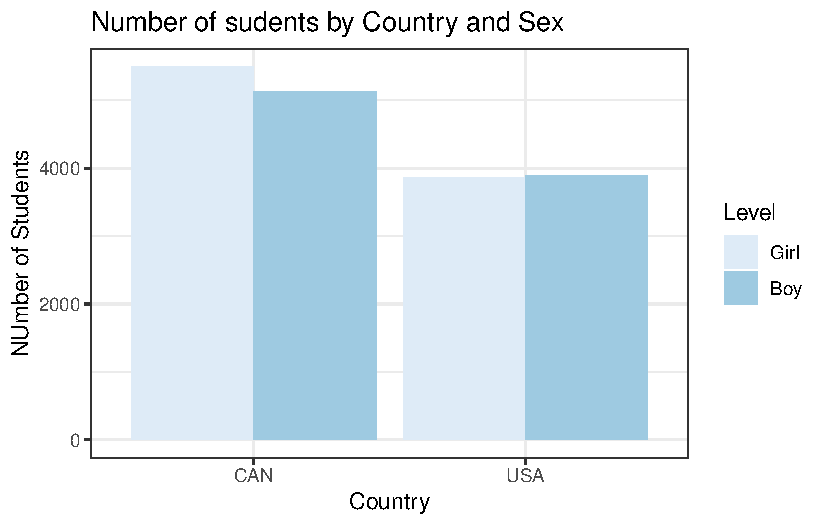
\includegraphics[keepaspectratio]{ESRM-6990V_files/figure-pdf/fig-Country-by-Sex-1.pdf}}

}

\caption{\label{fig-Country-by-Sex}Number of sudents by Country and Sex}

\end{figure}%

\begin{figure}

\centering{

\pandocbounded{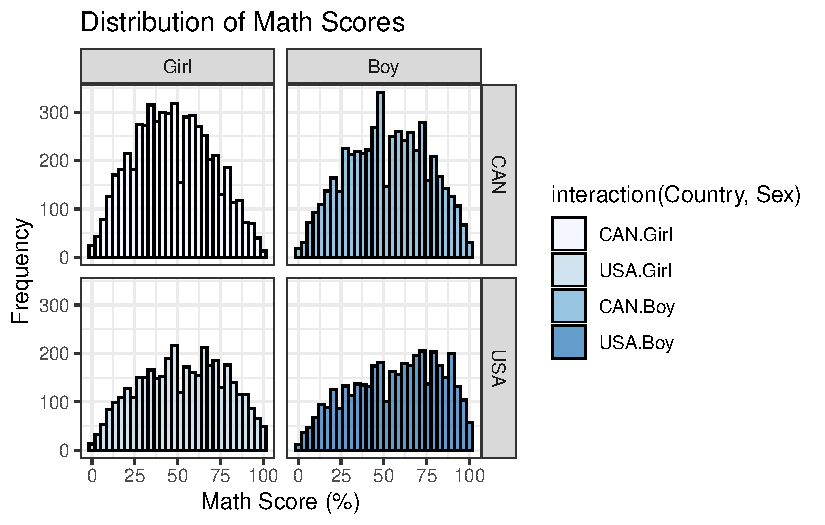
\includegraphics[keepaspectratio]{ESRM-6990V_files/figure-pdf/fig-dist-of-math-score-1.pdf}}

}

\caption{\label{fig-dist-of-math-score}Histogram of the Distribution of
Math Scores}

\end{figure}%

\begin{figure}

\begin{minipage}{0.50\linewidth}

\centering{

\pandocbounded{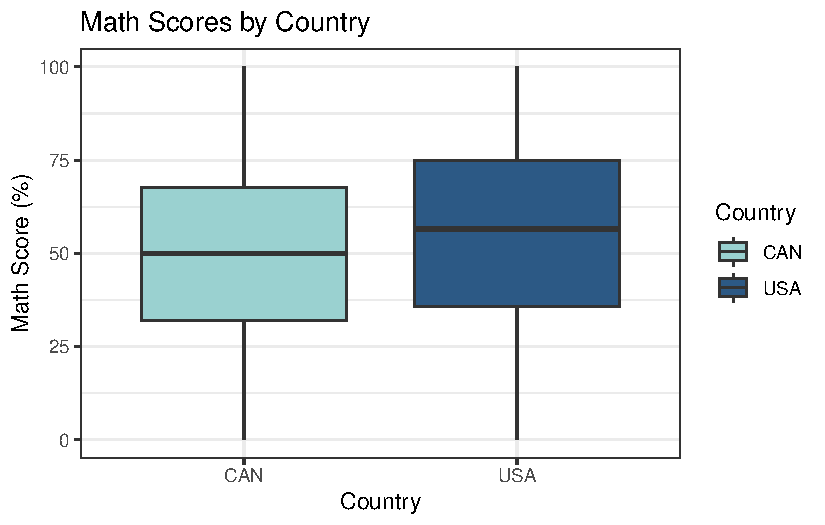
\includegraphics[keepaspectratio]{ESRM-6990V_files/figure-pdf/fig-dist-of-math-score-country-sex-home-support-1.pdf}}

}

\subcaption{\label{fig-dist-of-math-score-country-sex-home-support-1}Boxplots
of the the Distribution of Scores by Country}

\end{minipage}%
%
\begin{minipage}{0.50\linewidth}

\centering{

\pandocbounded{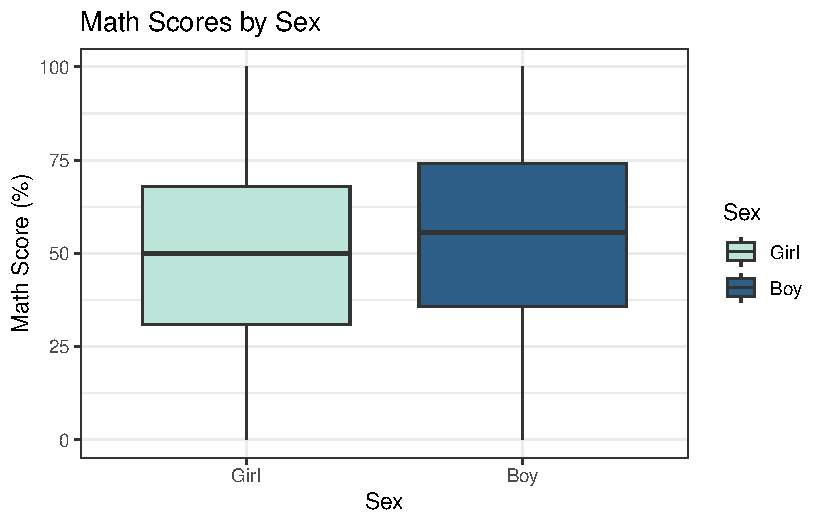
\includegraphics[keepaspectratio]{ESRM-6990V_files/figure-pdf/fig-dist-of-math-score-country-sex-home-support-2.pdf}}

}

\subcaption{\label{fig-dist-of-math-score-country-sex-home-support-2}Boxplots
of the the Distribution of Scores by Sex}

\end{minipage}%
\newline
\begin{minipage}{0.50\linewidth}

\centering{

\pandocbounded{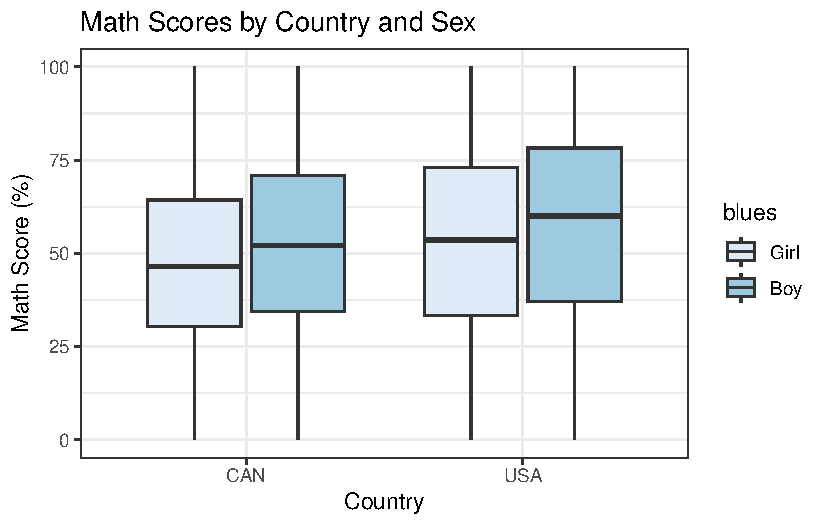
\includegraphics[keepaspectratio]{ESRM-6990V_files/figure-pdf/fig-dist-of-math-score-country-sex-home-support-3.pdf}}

}

\subcaption{\label{fig-dist-of-math-score-country-sex-home-support-3}Boxplots
of the the Distribution of Scores by Country and Sex}

\end{minipage}%
%
\begin{minipage}{0.50\linewidth}

\centering{

\pandocbounded{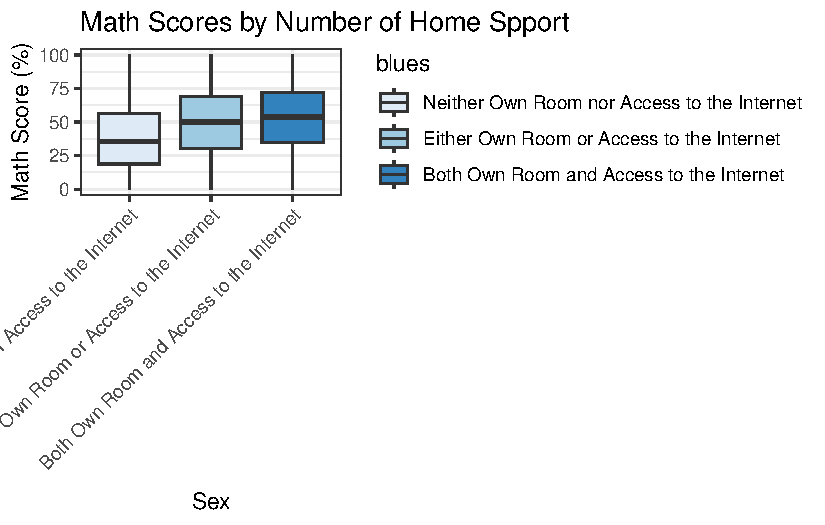
\includegraphics[keepaspectratio]{ESRM-6990V_files/figure-pdf/fig-dist-of-math-score-country-sex-home-support-4.pdf}}

}

\subcaption{\label{fig-dist-of-math-score-country-sex-home-support-4}Boxplots
of the the Distribution of Scores by Home Support}

\end{minipage}%

\caption{\label{fig-dist-of-math-score-country-sex-home-support}Boxplots
of the the Distribution of Scores by Country, Sex and Home Support}

\end{figure}%

\begin{figure}

\centering{

\pandocbounded{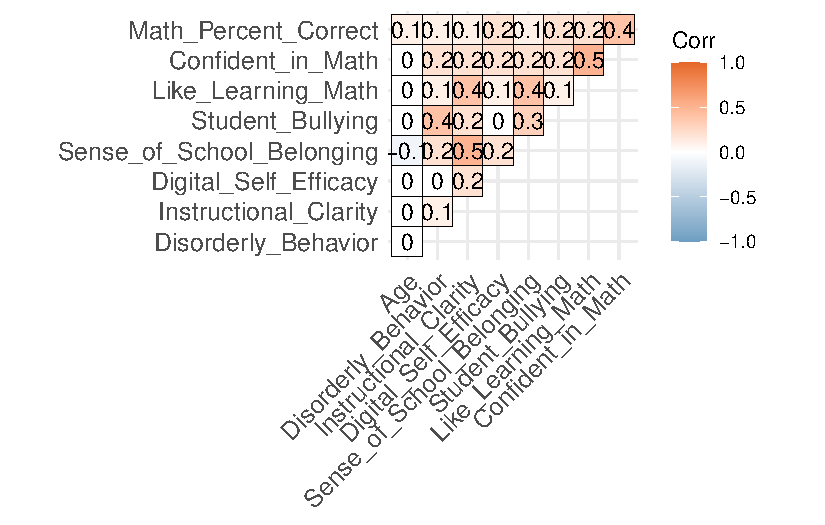
\includegraphics[keepaspectratio]{ESRM-6990V_files/figure-pdf/fig-Correlations-1.pdf}}

}

\caption{\label{fig-Correlations}Correlation Heatmap for Student-Level
Analysis}

\end{figure}%

\paragraph{Regression Analysis}\label{regression-analysis}

A step-wise regression model was estimated to evaluate whether the
independent variables \emph{(Country, Sex, Age, Disorderly\_Behavior,
Instructional\_Clarity, Digital\_Self\_Efficacy, Student\_Bullying,
Like\_Learning\_Math, Confident\_in\_Math, and
Number\_of\_Home\_Study\_Supports)} could predict the dependent
variable, \emph{Math\_Percent\_Correct} . The linear relationship
between independent variables and math score was found to be
statistically significant \(F(11, 18357) = 439.39,\ p < .001\). As shown
in Figure~\ref{fig-Correlations}, the correlations between the
predictors and math score were in the moderate to low range.
Appoximately \(21\%\) of the total variation in math percent score was
account for by its linear relationship with the predictors,
\(R^2 = .21,\ R^2_{adj}=.21\). Among the predictors, instructional
clarity had a statistically non-significant and negative effect on math
percentage value \((\beta = -.16,\ p < .001)\), suggesting that greater
instructional clarity was not associated with higher math percent values
in this model over and above all other predictors. The effect of Country
(U.S.A.) was statistically significant and positive
\((\beta = 5.58,\ p < .001)\), suggesting that holding all other
predictors unchanged, 4th grade students scored 5.58\% higher than those
in Canada. The effect of Sex (boy) was also statistically significant
and positive \((\beta = 2.01,\ p < .001)\), suggesting that controlling
for all other predictors, boys in the 4th grade scored 2.01\% higher
than girls. Interestingly, Like\_Learning\_Math was found to have
statistically significant and negative effect on math percent score
\((\beta = -.97,\ p < .001)\). This suggests that partialling out the
effects of all other predictors, and a unit increase in a student
whether a student likes learning math results in a -0.97\% decrease in
math percent score. All other predictors in the model had a
statistically significant and positive effect on math percent score.
This suggests that holding all other predictirs unchanged, an increase
in their respective values is expected lead to an increase in math
percentage score. The details of the results from the step-wise analysis
are presented in Table~\ref{tbl-Initial-regression-for-student-data}.
The predictor Confident\_in\_Math had the largest effect on the math
percent score followed by Number\_of\_Home\_Study\_Supports\_Either
\textbf{?@tbl-Initial-regression-for-student-data-4}. The predictors
used in this analysis do not exhibit multicollinearity as shown in
\textbf{?@tbl-Initial-regression-for-student-data-3}. A look at the
residual plots in Figure~\ref{fig-residual-std_reg_initial} show a
slight non-linearity with possible non-normality from the Q-Q plot.

\begin{longtable}[t]{lrrrr}

\caption{\label{tbl-Initial-regression-for-student-data}Student-Level
Regression Analysis}

\tabularnewline

\toprule
term & estimate & std.error & statistic & p.value\\
\midrule
(Intercept) & -35.487 & 4.634 & -7.658 & 0.000\\
CountryUSA & 5.584 & 0.346 & 16.123 & 0.000\\
SexBoy & 2.006 & 0.320 & 6.279 & 0.000\\
Age & 1.112 & 0.437 & 2.546 & 0.011\\
Disorderly\_Behavior & 0.603 & 0.102 & 5.903 & 0.000\\
\addlinespace
Instructional\_Clarity & -0.164 & 0.092 & -1.779 & 0.075\\
Digital\_Self\_Efficacy & 1.054 & 0.087 & 12.060 & 0.000\\
Student\_Bullying & 1.021 & 0.097 & 10.582 & 0.000\\
Like\_Learning\_Math & -0.968 & 0.098 & -9.892 & 0.000\\
Confident\_in\_Math & 4.773 & 0.094 & 50.695 & 0.000\\
\addlinespace
Number\_of\_Home\_Study\_SupportsEither Own Room or Access to the Internet & 8.055 & 0.990 & 8.140 & 0.000\\
Number\_of\_Home\_Study\_SupportsBoth Own Room and Access to the Internet & 10.088 & 0.965 & 10.451 & 0.000\\
\bottomrule

\end{longtable}

\begin{longtable}[t]{rrrrrrrrrrrr}

\caption{\label{tbl-Initial-regression-for-student-data}Student-Level
Regression Analysis}

\tabularnewline

\toprule
r.squared & adj.r.squared & sigma & statistic & p.value & df & logLik & AIC & BIC & deviance & df.residual & nobs\\
\midrule
0.208 & 0.208 & 21.298 & 439.394 & 0 & 11 & -82242.15 & 164510.3 & 164611.9 & 8326823 & 18357 & 18369\\
\bottomrule

\end{longtable}

\begin{longtable}[t]{lrrr}

\caption{\label{tbl-Initial-regression-for-student-data}Student-Level
Regression Analysis}

\tabularnewline

\toprule
 & GVIF & Df & GVIF\textasciicircum{}(1/(2*Df))\\
\midrule
Country & 1.185 & 1 & 1.088\\
Sex & 1.033 & 1 & 1.017\\
Age & 1.174 & 1 & 1.084\\
Disorderly\_Behavior & 1.160 & 1 & 1.077\\
Instructional\_Clarity & 1.254 & 1 & 1.120\\
\addlinespace
Digital\_Self\_Efficacy & 1.123 & 1 & 1.060\\
Student\_Bullying & 1.213 & 1 & 1.102\\
Like\_Learning\_Math & 1.551 & 1 & 1.245\\
Confident\_in\_Math & 1.508 & 1 & 1.228\\
Number\_of\_Home\_Study\_Supports & 1.039 & 2 & 1.010\\
\bottomrule

\end{longtable}

\begin{longtable}[t]{lr}

\caption{\label{tbl-Initial-regression-for-student-data}Student-Level
Regression Analysis}

\tabularnewline

\toprule
 & Estimate\\
\midrule
Intercept & -0.194\\
Country\_USA & 0.117\\
Sex\_Boy & 0.042\\
Age & 0.018\\
Disorderly\_Behavior & 0.042\\
\addlinespace
Instructional\_Clarity & -0.013\\
Digital\_Self\_Efficacy & 0.084\\
Student\_Bullying & 0.077\\
Like\_Learning\_Math & -0.081\\
Confident\_in\_Math & 0.409\\
\addlinespace
Number\_of\_Home\_Study\_Supports\_Either & 0.168\\
Number\_of\_Home\_Study\_Supports\_Both & 0.211\\
\bottomrule

\end{longtable}

\begin{figure}

\centering{

\pandocbounded{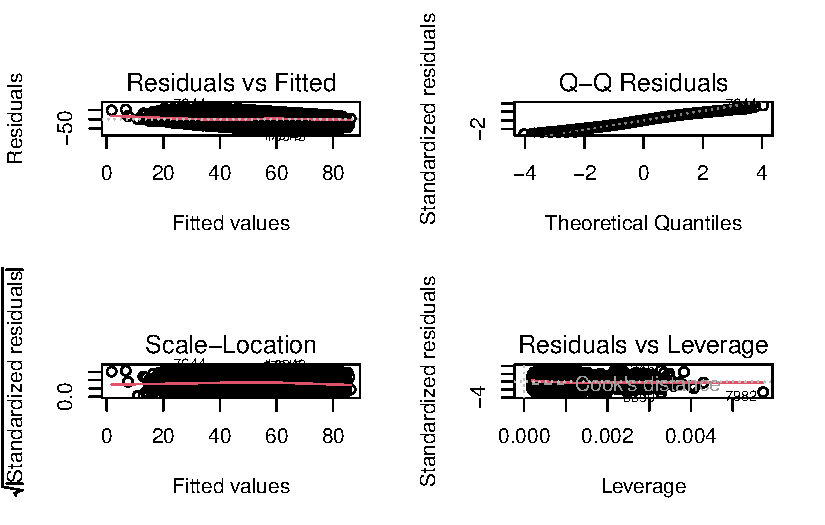
\includegraphics[keepaspectratio]{ESRM-6990V_files/figure-pdf/fig-residual-std_reg_initial-1.pdf}}

}

\caption{\label{fig-residual-std_reg_initial}}

\end{figure}%

\subparagraph{Difference-in-Difference Analysis on Combinations of Sex
and
Country}\label{difference-in-difference-analysis-on-combinations-of-sex-and-country}

This section of the analysis focuses on whether there are sex and/or
country specific differences in the performance of the 4th grade
students on the TIMSS math test. To do this, a
differences-in-differences analysis was performed on various
combinations of the country and sex variables. From
Table~\ref{tbl-Differences-in-Differences-tables} and
Figure~\ref{fig-Differences-in-Differences-fiqures}, it can be observed
that holding all other predictors unchanged, the predicted average math
percent value for a typical 4th grade student in the U.S.A is higher
than in Canada. Also, a typical Canadian or U.S.A 4th grade boy seem to
have a higher predicted average math percent score than their girl
counterparts. A marginal contrast analysis
(\textbf{?@tbl-Differences-in-Differences-tables-1}) was further
performed to evaluate if these differences were statistically
significant. This analysis revealed that the differences in predicted
scores across all combinations of sex and country were statistically
significant. In the U.S.A, boys had significantly higher predicted math
scores than girls
\((\text{difference}= 2.01,\ 95\%  \text{ CI } [1.38, 2.63],\ t(18357) = 6.28,\ p < .001)\).
Boys in Canada also had a significantly higher predicted math scores
than
girls\((\text{difference}= 2.01,\ 95\%  \text{ CI } [1.38, 2.63],\ t(18357) = 6.28,\ p < .001)\).
When comparing the average predicted scores of girls in the U.S.A. to
those in Canada, the girls in the U.S.A had a significantly higher score
\((\text{difference}= 5.58,\ 95\%   \text{ CI } [4.91, 6.26],\ t(18357) = 16.12,\ p < .001)\).
Similarly, girls in the U.S.A. also outperformed the boys in Canada
\((\text{difference}= -3.58,\ 95\%   \text{ CI } [–4.51, –2.65],\ t(18357) = -7.53,\ p < .001)\).
Additionally, boys in the U.S.A scored significantly higher than the
boys in Canada
\((\text{difference}= 5.58,\ 95\%   \text{ CI } [4.91, 6.26],\ t(18357) = 16.12,\ p < .001)\).
In the same vein, boys in the U.S.A. also outperformed the girls in
Canada by the largest margin
\((\text{difference}= 7.59,\ 95\%   \text{ CI } [6.67, 8.51],\ t(18357) = 16.25,\ p < .001)\).

These findings suggest that while gender differences exist, the national
level factors may play a more substantial role in the TIMSS math percent
score of 4th grade students. Further research should explore some
potential national level contributors like curriculum standards.

\begin{longtable}[t]{llrrrrrr}

\caption{\label{tbl-Differences-in-Differences-tables}Differences-in-Differences
Analysis}

\tabularnewline

\toprule
Sex & Country & Mean & SE & CI\_low & CI\_high & t & df\\
\midrule
Girl & CAN & 45.416 & 0.400 & 44.632 & 46.199 & 113.611 & 18357\\
Girl & USA & 51.000 & 0.422 & 50.172 & 51.828 & 120.766 & 18357\\
Boy & CAN & 47.422 & 0.404 & 46.630 & 48.214 & 117.353 & 18357\\
Boy & USA & 53.006 & 0.422 & 52.179 & 53.833 & 125.643 & 18357\\
\bottomrule

\end{longtable}

\begin{longtable}[t]{llrrrrrrr}

\caption{\label{tbl-Differences-in-Differences-tables}Differences-in-Differences
Analysis}

\tabularnewline

\toprule
Level1 & Level2 & Difference & SE & CI\_low & CI\_high & t & df & p\\
\midrule
Girl, USA & Girl, CAN & 5.584 & 0.346 & 4.905 & 6.263 & 16.123 & 18357 & 0\\
Boy, CAN & Girl, CAN & 2.006 & 0.320 & 1.380 & 2.633 & 6.279 & 18357 & 0\\
Boy, USA & Girl, CAN & 7.590 & 0.467 & 6.675 & 8.506 & 16.249 & 18357 & 0\\
Boy, CAN & Girl, USA & -3.577 & 0.475 & -4.509 & -2.646 & -7.527 & 18357 & 0\\
Boy, USA & Girl, USA & 2.006 & 0.320 & 1.380 & 2.633 & 6.279 & 18357 & 0\\
\addlinespace
Boy, USA & Boy, CAN & 5.584 & 0.346 & 4.905 & 6.263 & 16.123 & 18357 & 0\\
\bottomrule

\end{longtable}

\begin{figure}

\centering{

\pandocbounded{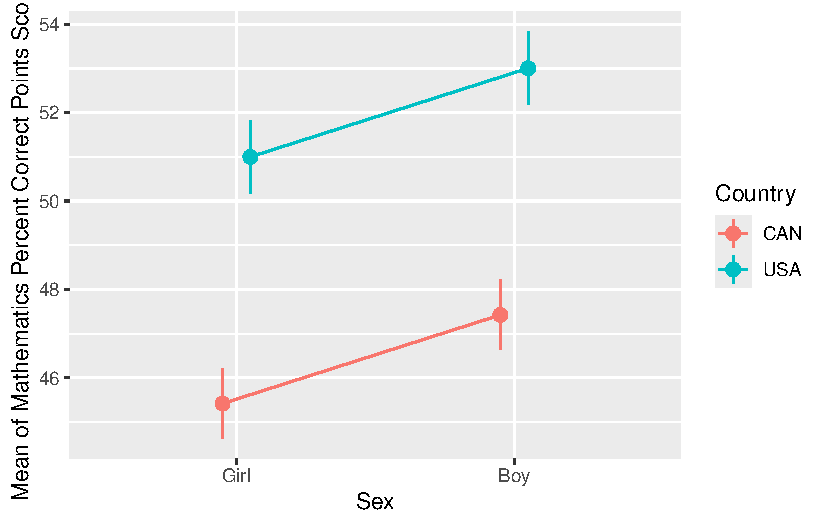
\includegraphics[keepaspectratio]{ESRM-6990V_files/figure-pdf/fig-Differences-in-Differences-fiqures-1.pdf}}

}

\caption{\label{fig-Differences-in-Differences-fiqures}Estimated
Marginal Means of Predicted Math Scores by Sex and Country}

\end{figure}%

\subsubsection{Teacher-Level Analysis}\label{teacher-level-analysis}

The dataset used in this contained a total of 18194 participants after
data cleaning. The dataset had a total of 538 variables but only 14 are
reported below:

\begin{itemize}
\item
  \textbf{Teacher\_ID:} Teacher Identifier
\item
  \textbf{Years\_Teaching:} Years teacher has been teaching
\item
  \textbf{Sex:} Sex/Gender of teacher (1: Female; 2: Male; 3: Other)
\item
  \textbf{Age:} Age of Teacher (1: Under 25; 2: 25--29; 3: 30--39; 4:
  40--49; 5: 50--59; 6: 60 or more)
\item
  \textbf{Level\_of\_Formal\_Educ:} Level of formal education teacher
  has completed (1: Did not complete Upper secondary education---ISCED
  Level 3; 2: Upper secondary education---ISCED Level 3 (have not
  completed postsecondary or tertiary education); 3: Post-secondary,
  non-tertiary education---ISCED Level 4; 4: Short-cycle tertiary
  education---ISCED Level 5; 5: Bachelor's or equivalent level---ISCED
  Level 6; 6: Master's or equivalent level---ISCED Level 7; 7: Doctor or
  equivalent level---ISCED Level 8)
\item
  \textbf{Class\_Size:} Number of students in the class.
\item
  \textbf{Homework\_Freq:} How often math homework is assigned (1: I do
  not assign mathematics homework; 2: Less than once a week; 3: 1 or 2
  times a week; 4: 3 or 4 times a week; 5: Every day)
\item
  \textbf{Tch\_Academic\_Success:} Scale score from the subscale
  measuring school emphasis on academic success-teacher.
\item
  \textbf{Safe\_Orderly\_Schools :} Scale score from the subscale
  measuring safe and orderly schools-teacher.
\item
  \textbf{Tch\_Job\_Satis :} Scale score from the subscale measuring
  teachers job satisfaction.
\item
  \textbf{Student\_not\_Ready:} Scale score from the subscale measuring
  teaching limited by student not ready.
\item
  \textbf{Tch\_Educ\_Math\_Major :} Teachers majored in education and
  mathematics (1: Major in Edu and Math; 2: Major in Edu but not Math;
  3: Major in Math but not Edu; 4: All other Majors; 5: No Formal Edu
  Beyond Upper Secondary).
\item
  \textbf{Math\_Instruction\_Hours:} Mathematics instruction hours per
  week
\item
  \textbf{Math\_Percent\_Correct}: Students' percent correct on the 2023
  TIMSS Math Achievement Test.
\end{itemize}

The scale scores reported were derived following several steps
including; item parameter estimation, item fit evaluation among others
(Yin and Reynolds 2024).

\paragraph{Data Preparation}\label{data-preparation-1}

As with the \texttt{Home\_Student} dataset, the data preparation for the
\texttt{Teacher\_Student} dataset started with renaming the original
variables with more descriptive names. After this, the dataset is
cleaned by removing any rows containing missing values resulting in a
final dataset with only complete cases as well as specifying categorical
variables and dropping any unused levels.

\paragraph{Descriptive Statistics}\label{descriptive-statistics-1}

The total sample size of the Canada and U.S.A. 4th grade students was
22806. However, due to non-response, the sample size used for this
analysis was 18369; 9351 girls and 9018 boys. There were more Canadian
4th Grade students compared to the U.S.A. in the sample
(Figure~\ref{fig-Country-by-Sex}). The overall mean age was 10 years
(S.D. = 0.390) and the average sample class score was 52\% (S.D. =
0.390). About 51\% of the entire sample was female with Canada
accounting for about 52\% of the total population of females. A
comprehensive summary of the sample information can be seen in
Table~\ref{tbl-sample-descriptives}. The distribution of the math scores
for each country and sex subgroup can be described asbimodal as shown in
Figure~\ref{fig-dist-of-math-score}. As shown in
Figure~\ref{fig-dist-of-math-score-country-sex-home-support}, it can be
observed that U.S.A students had a higher Math score average with boys
also having a higher average score. Students who had access to both
their own rooms and internet access seemed to have a better average
score compared to those who had neither
(Figure~\ref{fig-dist-of-math-score-country-sex-home-support-4}).

\phantomsection\label{refs}
\begin{CSLReferences}{1}{0}
\bibitem[\citeproctext]{ref-yin2024}
Yin, Liqun, and Katherine Reynolds. 2024. {``Creating and Interpreting
the TIMSS Context Questionnaire Scales.''}
\url{https://doi.org/10.6017/lse.tpisc.timss.rs2550}.

\end{CSLReferences}




\end{document}
